%!TEX TS-program = xelatex
%!TEX root = ../../maxwell2018thesis.tex

\chapter[Information Retrieval]{Information Retrieval:\\History and Background}\label{chap:ir}

\begin{quote}
    \emph{``Information Retrieval deals with the representation, storage, organisation of and access to information items.''}
    \attrib{\citealp{baezayates1999modern_ir}}
\end{quote}

Without the availability of retrieval systems today, finding information would be a much more difficult task. Considering how easy the systems that we use on a daily basis are so straightforward to use, one might be forgiven in thinking that they were easy to develop.

In reality, this could not be further from the truth. Central to how these retrieval systems operate is the work that has been undertaken in the field of~\gls{ir} over a number of decades. In this chapter, we provide a provide a brief summary of the field of~\gls{ir} -- from the first experiments up to the present day (Section~\ref{sec:ir:history}) -- and then examine the key concepts that are assumed within~\gls{ir} systems and experimentation today. From then, we begin to discuss the different models and measures that are commonly used within the field to evaluate the effectiveness of systems and users, all with an emphasis on how one can consider search stopping within them.

\section[A (Brief) History]{A (Brief) History of Information Retrieval}\label{sec:ir:history}
Given the abundance of contemporary, computer-based technologies readily available in our lives today, one might be forgiven in thinking that the humble \emph{book} is in itself a technological development. The book provides us with the means of storing knowledge and information, with a book's ability to preserve information through the ages not going unnoticed~\citep{hedstrom1997digital_preservation}. With approximately 130 million unique titles in existence as of 2010\footnote{This figure is estimated and presented on the \emph{Google Books Search blog}, now archived, at \url{http://booksearch.blogspot.co.uk/}.}, individuals would access a \emph{library} to acquire the book(s) -- and subsequent knowledge that they possess.

\subsection{Libraries, Indexing and Punchcards}
The field of~\gls{ir} has transformed the way in which we access information. Back in the early 20\textsuperscript{th} century, an individual would access books in their local library, with books organised by means of a classification system. A popular example of such a system is the \emph{Dewey Decimal System}~\citep{dewey1891dcs}. By examining the classification system, an individual would then be able to navigate themselves to the relevant area of the library floor to find their book. Such an approach -- while acceptable at the time -- was an inconvenience. Due to the comparatively high costs involved, information seekers would limit themselves to perhaps a small number of questions~\citep{sanderson2012history_of_ir}.



\begin{figure}[t!]
    \centering
    \resizebox{1\hsize}{!}{
    
\includegraphics{figures/ch2-search_integration.png}}
    \caption[Search Integration within Windows 10]{An illustrative example of how search has become integrated within computer operating systems. In this screenshot, the query \texttt{glasgow university} has been issued to \emph{Bing}, through the \emph{Microsoft}'s \emph{Windows 10} desktop interface. This search interface allows both searching locally for files on disk, and for external web search queries.}
    \label{fig:ch2-search_integration}
\end{figure}

\subsection{The Rise of Computers}

\subsection{The World Wide Web}

\section{Information Retrieval Basics}

\subsection{The Cranfield Paradigm}

\section{Retrieval Models}

\subsection{Boolean Retrieval}

\subsection{Probabilistic Retrieval}

\section{System/User Evaluation}

\subsection{Precision-at-k}

\subsection{Rank-Biased Precision}

\subsection{INST}


\section{Chapter Summary}
- ir is a diverse field
- lots of models and measures
    - they encode some form of stopping rules within them.
    - in the next chapter, we start to look at stopping rules.


%====== OLD ======%
% \section{A (Brief) History of Information Retrieval}
%
% sought to make finding information easy.
% first place one think of would be a library and systems like the dewey decimal system made it easier to find books.
% but as technology developed, computers appeared, and so too did the rise of information stored electronically.
%
% without retrieval, there is no information.
%
% so much out there, it's a proverbial needle in a haystack? IR is the study of assisting people to find that proverbial needle in a wealth of information. so how did we get to where we are today? this section provides a brief overview of the major technological advancements in finding that all important relevant information, before we delve deeper into the the many approaches that have been used in the development of IR over the decades as a research area.
%
% contrary to popular belief, (maybe), search has been around long before the advent of the World Wide Web, that we synonymously associate with search today, throughs search engines like google and bing.
%
% \subsection{Library Search}
%
% \subsection{The Rise of Computers}
%
% \subsection{The World Wide Web}
%
% dominate over existing protocols, such as gopher
% \url{https://ils.unc.edu/callee/gopherpaper.htm}
%
% gopher used a telephone directory style, menu-based system.
% better ways of presenting information, especially as the amount of information we generate grew.
%
% \begin{quote}
%     December, 1993
%     National Center for Supercomputing Applications (NCSA)
% The JumpStation is a WWW Form for finding other WWW Pages. At present it is in its Alpha state, and cannot be relied upon too heavily. Problem: The current problem is the search speed (it is SLOW!).
%     \url{https://web.archive.org/web/20010620073530/http://archive.ncsa.uiuc.edu/SDG/Software/Mosaic/Docs/old-whats-new/whats-new-1293.html}
% \end{quote}
%
% - acted much like a telephone directory.
% - content was separated out into different categories.
% - this was soon seen to be too much, as the exponential growth of WWW content made this approach difficult to navigate and find what you were looking for.
% - there needed to be a better way -- the query box.
% - we discuss much of the techniques developed over time in the following section, but to give a brief history...
%     - the search box allowed for the first time online people to enter their own queries.
%     - original search systems were poor in terms of retrieval, looked up terms in documents and matched them.
% - then came google...
%     - pagerank algorithm
%     - for the first time, people exploited the idea that links between pages could provide information about the relevancy or importance of given documents.
%
% Search as embodied by the text box and keyword has framed our
% understanding of what the Web is [145] ] m. c. schraefel, “Building knowledge: What’s beyond keyword search?,” Computer,
% vol. 42, no. 3, pp. 52–59, 2009.
%
% \begin{figure}[ht]
%     \centering
%
%     \resizebox{1\hsize}{!}{
%     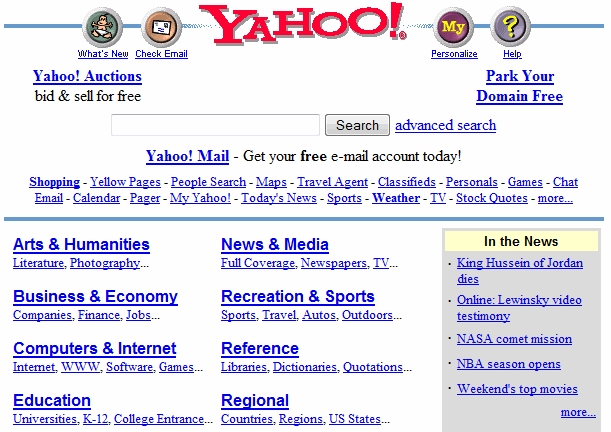
\includegraphics{figures/ch2-yahoo.png}}
%     \caption[Yahoo! Homepage]{Old search engine -- Yahoo! Note the directory-based listings, with the recent addition (at the time) of a search box, allowing users to enter their own queries}
%
%     \label{fig:ch2-mclaren}
% \end{figure}
%
% some of the first advancements were....
%     - library systems
%
% search
% library systems
% computers
% the internet and world wide web
%
%
% In this chapter, we provide a general background on the fundamental concepts established within the field of~\gls{ir}, along with definitions that are required to understand the topics that we explore later in this thesis. We cover a variety of topics in this chapter, from basic~\gls{ir} concepts, models and evaluation methodologies that are commonly deployed. Refer to Chapter~\ref{chap:sim_background} for more information on simulation; specifically, simulation within~\gls{ir}~\gls{computer}.
%
%     \begin{quote}
%         \Large
%         ``But perhaps the key technology that took the Web from a useful supplement of current information practice to become the default communication medium is search.''
%         \attrib{Max Wilson}
%     \end{quote}
%
% \section{Cranfield}
% The Cranfield paradigm was designed in the early 1960s when information access was via Boolean
% queries against manually indexed documents and there was (virtually) no text online. Cyril
% Cleverdon, Librarian of the College of Aeronautics, Cranfield, England, built a test collection that
% modeled university researchers, including abstracts of aeronautical papers, one-line queries based
% on questions gathered from the researchers, and complete relevance judgments for each query
% submitted by these users. The idea of carefully modeling some user application continued with
% Prof. Gerard Salton and the SMART collections, such as searching MEDLINE abstracts using real
% questions submitted to MEDLINE, or searching full text TIME articles with real questions from
% several sources, etc. A 1969 paper by Michael Lesk and Salton used experiments on the ISPRA
% collection to show that relevance judgments made by a person who was not the user would still
% allow valid system comparison, a precursor to the paper by Ellen Voorhees in SIGIR 1998.
% Implementation of the Cranfield paradigm has undergone extensive modifications over the years in
% TREC and other evaluation forums as the data and tasks have gotten more complex. However it
% still stands as the model of choice, both for these (mostly) academic evaluations and at least
% partially for commercial evaluations, especially for straight-forward searching tasks where clicks
% and dwell times can be used to predict relevance. However the world of information access has
% exploded in recent years to encompass online shopping, social networking, personal desktop
% organization, etc. Is it time to have a new paradigm, and if so, how do we ensure that information
% retrieval evaluation remains scientifically valid?
%
%
% \citep{harman2010cranfield}
%
% \section{Basic Principles}
% tasked to find information in a series of documents. modern day information retrieval concerns retrieval of relevant documents via some retrieval system with the use of a query issued by a user.
%
% basic principles of IR -- what a query is, what a document is, what a retrieval system is... absolute basics.
% then we can talk about the history of IR, followed by a discussion on the more advanced stuff, like what the models are that are used in retrieval systems, how we evaluate how good systems are, for example.
%
% \section{Stemming?}
%
% \section{Information Retrieval Tasks}
% \section{Retrieval Models}
% \subsection{Boolean Model}
% \subsection{Vector Space Model}
% \subsection{Probabilistic Models}
% \subsection{Language Models}
% \section{Experimental Methodologies}
% \subsection{System-Orientated Evaluation}
% \subsection{User-orientated Evaluation}
% \section{Evaluating Retrieval Effectiveness}
% \subsection{Recall}
% \subsection{Precision}
% \subsection{Mean Average Precision}
% \subsection{F-Measure}
% \subsection{Rank-Biased Precision}
% \subsection{Other measures}
% \section{Interactive Information Retrieval}
%
% \subsection{User Studies: The Basics}
% \subsection{IIR Evaluation}
% \section{Chapter Summary}